\paragraph{Tijdsduur}
\begin{figure}[H]
  \centering
  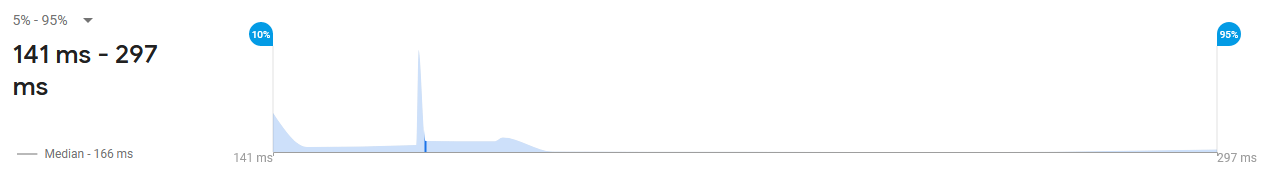
\includegraphics[height=0.1\textheight]{notificatiesDuratieCross.png}
  \caption{Overzicht tijdsduur aanmaken notificaties bij React Native.}
\end{figure}
Tijdens het meten van de duur voor het aanmaken van een notificatie, is er net zoals bij native 
10 keer een notificatie aangemaakt. Na 10 keer een notificatie aan te maken is er 
een gemiddelde duur van 166ms en met een minimum en 
maximum van 141ms en 297ms voor het aanmaken van een notificatie.

\paragraph{CPU \& geheugen}
\begin{figure}[H]
  \centering
  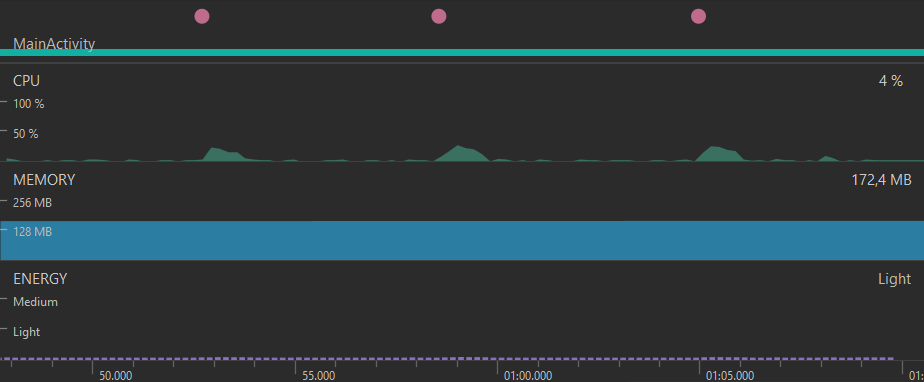
\includegraphics[height=0.25\textheight]{notificatiesPerformantieCross.png}
  \caption{Overzicht CPU en geheugen gebruik tijdens aanmaken notificaties bij React Native.}
\end{figure}
Op de grafiek is te zien dat het CPU gebruik van de applicatie wanneer deze inactief is, rond de 4\% ligt. 
Daarnaast is het duidelijk zichtbaar wanneer een notificatie wordt aangemaakt. De piek van het CPU gebruik lag 
gemiddeld op 28\% en schommelde tussen de 25\% en 30\%. Het geheugen blijft in tegenstelling tot de CPU 
wanneer de applicatie inactief en actief is, rond de 172MB hangen, met verschillen van maximum 0,5MB. 
Er is geen merkbaar verschil in het geheugen wanneer een notificatie wordt aangemaakt.
